% !TeX root = ../../tesis.tex

\subsection{El Futuro de Apimetro}
\label{subsec:futuro-apimetro}

\texttt{Apimetro} se define no solo como una herramienta técnica, sino como un
proyecto de \textbf{software libre} comprometido con la democratización de los
datos de movilidad en la \zmvm. Bajo la premisa de soberanía tecnológica, el
proyecto se encuentra en una fase de expansión activa, proyectando un
crecimiento significativo en su cobertura y capacidades analíticas en los
próximos meses \citep{cabrera2025apimetro}. Para facilitar la transparencia, el
estudio y la redistribución del conocimiento generado, el ecosistema de
\texttt{Apimetro} se articula a través de cuatro plataformas principales:

\paragraph{1. Página Oficial (apimetro.dev):} Es el punto de entrada principal
para usuarios y desarrolladores. En este portal se aloja la documentación
interactiva (Swagger UI), el estado de salud del servidor de producción y los
accesos rápidos a los recursos de la API masiva.

\begin{figure}[htbp]
  \centering
  \includegraphics[width=0.85\textwidth]{Figures/Cap3/PantallaInicialApimetro.png}
  \caption{Interfaz principal del portal \url{apimetro.dev}.}
  \label{fig:screenshot-web}
\end{figure}

\paragraph{2. Repositorio de Código en GitHub:} Constituye el núcleo técnico del
proyecto. Aquí se encuentra el código fuente en \textbf{Go}, los motores de
ingesta \textbf{ETL} y las configuraciones de despliegue mediante
\textbf{Docker}. El repositorio está bajo una licencia
\textit{Business Source License 1.1}, la cual garantiza su uso gratuito para
fines académicos, de investigación y del sector público, con una transición
automática a la licencia \textit{Apache 2.0} en abril de 2029
\citep{cabrera2025apimetro}.

\begin{figure}[htbp]
  \centering
  \includegraphics[width=0.85\textwidth]{Figures/Cap3/PantallaInicialApimetroGithub.png}
  \caption{Estructura del c{\'o}digo fuente y control de versiones en GitHub.}
  \label{fig:screenshot-repo}
\end{figure}

\paragraph{3. Comunidad de Desarrollo (Discussions):} Espacio dedicado a la
colaboración abierta y la gobernanza del proyecto. A través de este canal, la
comunidad puede proponer nuevas funcionalidades, reportar incidencias en los
trazos de transporte o discutir la integración de nuevos sistemas de la Zona
Metropolitana, fomentando una construcción colectiva de la infraestructura de
datos.

\begin{figure}[htbp]
  \centering
  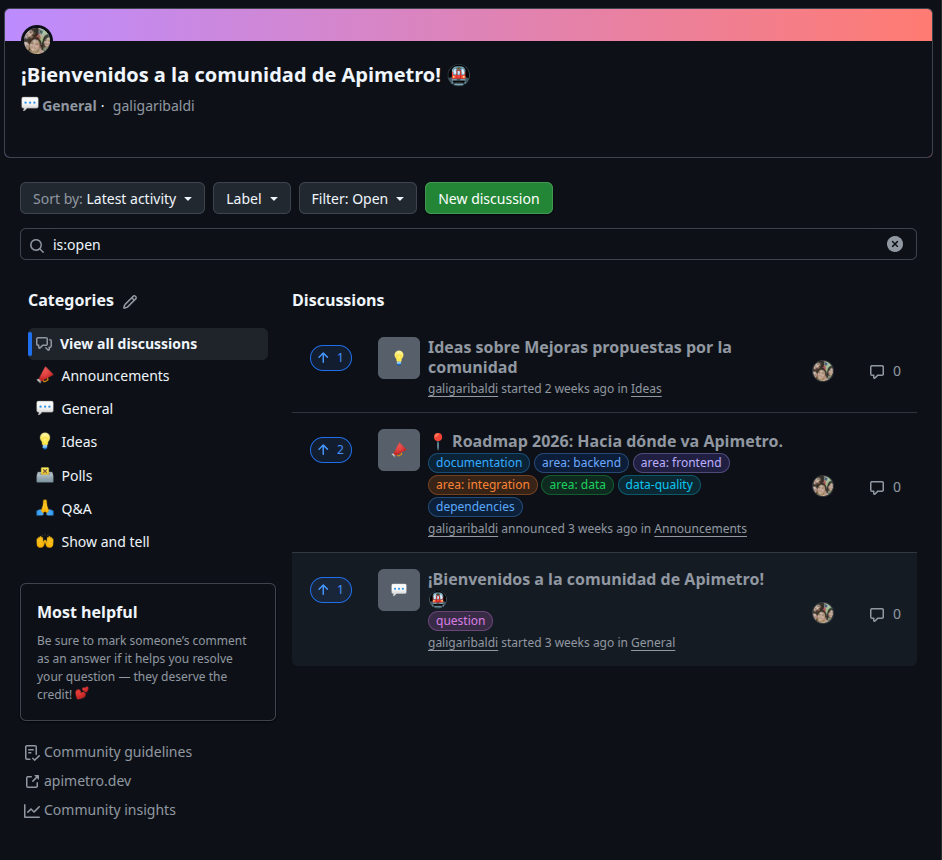
\includegraphics[width=0.85\textwidth]{Figures/Cap3/PantallaInicialComunidadApimetro.png}
  \caption{Foro de discusi{\'o}n y colaboraci{\'o}n de la comunidad Apimetro.}
  \label{fig:screenshot-discussions}
\end{figure}

\paragraph{4. Wiki de Apimetro:} Centro de documentación técnica profunda donde
se detallan las guías de implementación, el diccionario de datos de las tablas
\texttt{SQL} y los procedimientos para replicar el motor de datos de forma local
utilizando el archivo \texttt{seed.sql}.

\begin{figure}[htbp]
  \centering
  \includegraphics[width=0.85\textwidth]{Figures/Cap3/PantallawikiApimetro.png}
  \caption{Repositorio de documentaci{\'o}n t{\'e}cnica y gu{\'i}as de implementaci{\'o}n.}
  \label{fig:screenshot-wiki}
\end{figure}

Esta infraestructura digital asegura que la investigación no termine con la
entrega de la tesis, sino que perdure como un \textbf{bien público tecnológico}
capaz de evolucionar y adaptarse a las dinámicas cambiantes de la movilidad
urbana en México \citep{fortin2016innovative}.
